\documentclass[12pt, a4paper]{report}
\usepackage[utf8]{inputenc}
\usepackage[swedish]{babel}
\usepackage{relsize}
\usepackage[backend=biber, style=numeric-comp, sorting=ynt]{biblatex}
\usepackage{csquotes}
\usepackage{graphicx}
\usepackage{titlesec}
\usepackage{titling}
\usepackage{pgf-pie}
\usepackage{hyperref}

\emergencystretch=1em

\setcounter{secnumdepth}{0}

\bibliography{bibliography.bib}
\addbibresource{biliography.bib}

\author{Eddie Englund}
\title{Linux vs Windows\\[0.2em]\smaller{}En djupgående analys av prestanda skillnader mellan Microsoft Windows och Manjaro Linux}
\date{VT 2020}

\renewcommand{\abstractname}{Abstract}
\renewcommand{\abstract}{Abstract}
\renewcommand*{\bibfont}{\small}


\begin{document}

\begin{titlepage}

    \maketitle

    \begin{center}

    
        
\includegraphics[width=0.15\textwidth]{nti}\par\vspace{1cm}

    {\scshape\LARGE NTI Gymnasiet Gärdet \par}
    \vspace{1cm}
    {\scshape\Large Examensarbete/Master Thesis, April 2020\par}
	\vspace{1.5cm}
    \textbf{
    Student: Eddie Englund, eddie.englund@elev.ga.ntig.se även eddie.englund@protonmail.com}
    \vspace{0.2cm}

    Handledare NTIG: Haris Kasumović, Haris.Kasumovic@ntig.se
    \vspace{0.1cm}

    Examinator NTIG: Haris Kasumović, Haris.Kasumovic@ntig.se
    
    \end{center}
\end{titlepage}


\section{Sammanfattning}\label{sum}

    \begin{abstract}

    \end{abstract}

\tableofcontents

\vspace{3cm}

    
\section{Inledning}


    I och med att världen blir mer och mer digitaliserad varje dag så är det inte konstigt att det finns en massiv marknad med olika alternativ för näst intill allting när det kommer till den digitaliserade värdlen. Allt från telefoner till hem datorer eller kanske till och med smart damsugare eller också en smart gräsklippare. Alla dessa digitaliserade mirakel har en sak gemensamt. Dem alla har ett operativ system.

    Världens mest kända operativsystem (inom allmenheten) är Microsoft Windows. Microsoft har en lång rad med olika verisioner av sitt operativ system\cite{windows}: Windows XP, Windows Vista, Windows 7[\dots] och deras senaste (och förmodligen sista) operativ system Windows 10.
     I alla Apple datorer så har man macOS, i deras telefoner har dom IOS och i deras nya Ipads så har dom iPadOS.
     Det finns faktisk ett tredje ``operativsystem''; Linux är en så kallad Kernel \cite{redhat} som är det man kan bygga ett operativsystem på. Linux har många olika operativsystem som är kallade för distributioner eller förkortat \textit{``distros''}. Linux är välkänt inom utväcklar värdlen eftersom att det är mycket vänligt för utvecklingsmiljöer men också eftersom att Linux har (offtast) en mycket god prestanda på maskiner med mindre processor kraft. På grund av detta så är bl.a: iPadOS, IOS, macOS, Android och näst intill allting annat som inte har så mycket processor kraft som t.ex en hiss. Men reflekterars Linux kraftiga prestanda på mindre starka maskiner med lite CPU kraft likadant på dom starka maskinerna? Är prestandan bättre på ``starka'' maskiner som kör Linux som sin kernel?


\section{Bakrund}

    Linux är inte operativsystem. Däremot, så är Linux det som kallas för en ``kernel''\cite{redhat}. Det är hjärtat av operativsystemet eller kanske lite bättre jämfört med hjärnan av operativsystemet. Kerneln är en typ av mellanhand, mellan mjukvaran och hårdvaran. Den hanterar minnet och processer men även också en del andra saker.

    Men eftersom att Linux är en kernel så finns det många så kallade distributioner/verisioner (operativsystem). Skillanderna på dem olika distributionerna kan variera högt, men offtast handlar dom största skillnaderna om vilka så kalladed ``repositories'' man använder för att distrubera mjukvara. Dessutom så kan det handla om villka filsystem man använder men också hur mycket eller hur lite förinstallerade program som finns när man installerar distrobutionen.
    
    Den distributionen som jag har valt att använda är Manjaro\cite{manjaro}. Manjaro är en så kallad \textit{Arch based distro}. Den är baserad på en annan distro som heter Arch Linux som ofta blir kallat för den bästa distron. Men, Manjaro gör det lättare att komma igång och så har Manjaro dom flesta fördelarna som Arch.

    Men den största skillnaden mellan Linux och Windows är att det inte är proprietär och har öppen källkod vilket betyder att vem som helst kan bidra med kod för att; göra kerneln eller distributionen bättre och lägga till fler användbara funktioner, men även också att fixa buggar. Öppen källkod har även en annan fördel och det är att koden oftast inte är så kallad \textit{``bloated''}, alltså att det finns kod eller funktioner som inte behövs eller att kod kvaliteten inte är bra. Detta leder till att prestandan på Linux är mycket hög. 
    
    Därför så vill jag ta reda på om prestandan mellan Linux (manjaro) och Microsoft Windows 10 har en uppenbar skillnad och om dom har det, varför? Jag vill dessutom veta vad konsensusen är kring Linux i utväcklar grupper/forum.
\subsection{Vad tror utvecklare?}

    För att ta reda på vad andra utvecklare har för hypotes/teori om prestandan mellan Linux i allmänhet och Windows 10, varför prestandan skulle vara annorlunda, vilket operativsystem dom föredrar och varför.  Så delades det runt ett formulär runt om kring olika programmerings/utvecklingsforum men även genom kontakter lyckats skicka vidare formuläret i proffesionella utvecklingsmiljöer.

    Notera att formuläret var skrivet på Engelska för att kunna nå ut till så många utvecklare så möjligt.


    \vspace{2.7cm}


    \large {Which operating system would have superior performance in tasks like, compiling code, executing code or even intensive workloads like working in a program  like blender or unity?}

    \vspace{.5cm}

    \normalsize I denna fråga så frågade vi olika utvecklare vad dom trode kring Linux. Tror dom att Linux eller Windows har bättre prestanda när det kommer till att kompilera/köra/använda olika applicationer/program


    \vspace{1cm}

    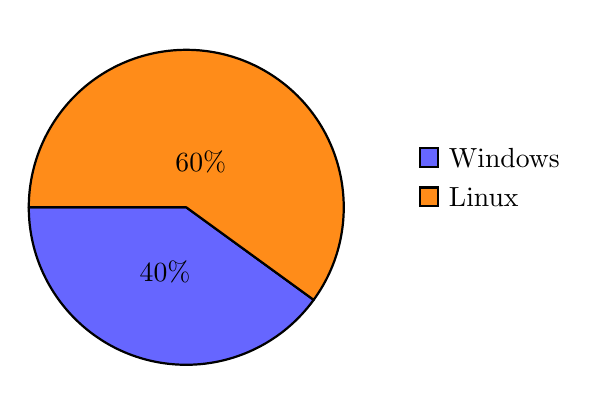
\begin{tikzpicture}
        \pie [rotate = 180, color = {blue!60, orange!90}, radius = 2, text = legend]
    {40/Windows,
     60/Linux}

    \end{tikzpicture}

    \cite{form}
    \vspace{3cm}

    \large{If you had the option to choose between Windows and Linux which one would you choose? (of course, you can choose any distro for Linux)}
    
    \vspace{.5cm}
    
    \normalsize I Denna fråga så frågar vi utvecklare vilket operativsystem dom skulle välja om dom hade chansen. Vi fick ett ganska fascinerande resultat. Om vi hade fått ett jämt antal svar så hade det varit en rak 50 50 på denna fråga men den tjugotredje personen som svarade på frågan valde Linux över Windows.

    \vspace{1cm}

    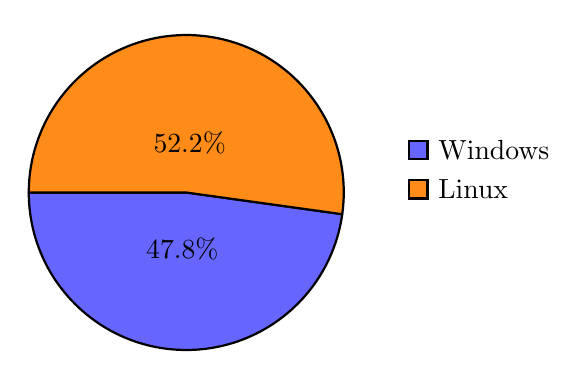
\begin{tikzpicture}
        \pie [rotate = 180, color = {blue!60, orange!90}, radius = 2, text=legend]
    {47.8/Windows,
     52.2/Linux}

    \end{tikzpicture}

    \cite{form}

    \vspace{1cm}


    \small{OBS! Det fanns några frågor som var alternativa, till exempel: att motivera sina svar.
    
    Vill ni läsa dessa motiveringar så finns dom här:} \smaller{\url{https://tinyurl.com/rccw2af}}


\section{Metod}

För att ta reda på om det finns prestanda skillnander mellan Windows och Linux (manjaro) så behöver vi först ta reda på en del saker.

\begin{enumerate}
    \item Vilket språk bör användas och varför?
    \item Vad bör man utföra för uppgift i programmet för att få machinerna att arbeta?
    \item Hur mäter vi prestandan?
    \item Hur kan vi verifera våra mätningar?
\end{enumerate}

Den första frågan ledde till ett ganska djupt hål eftersom att det finns extremt många programmerings språk. Bara för att nämna ett par: Java, Javascript, Python, C, C++, C\#, Haskell, Ruby, Rust, mm. Okej, så vi har en hel del olika språk.

Så vi kan börja med utesluta dem långsamma språken. Direkt då så utesluts: Ruby, Javascript och Python. Vi viller heller inte ha språk som måste bli \textit{interpreted} i runtime. Då försvinner Java. Detta eftersom att Java har det som kallas för \textit{JVM} vilket är kort för ``Java Virtual Machine''. Detta var skapat för att ha ett kompabilitets lager så att man ska kunna köra Java program på alla datorer oavsätt operativsystem. Därefter så vore det också bra om man kan köra/skriva språket på Linux utan att lägga till extra kompabilitets lager. Då försvinner C\# eftersom att för att köra det på Linux så behöver man det som kallas för ``.Net Core'' vilket fungerar som JVM och av samma anledning som Java så vill vi inte ha det. Nu har vi endast C, C++ och rust kvar och eftersom att jag har lite erfarenhet med rust och eftersom att rust inte är lika svårt när det kommer till saker som minnes hantering så slutade det med att jag valde Rust som språk.


Så nu har vi ett språk som vi vet är snabbt, stabilt och kan köras på flera maskiner (efter kompilering till den plattformen). Vad bör programmet utför för uppgift? Ett problem som uppstog när jag först försökte fylla en vector med 1 gigabyte utav integers och sedan loopade programmet för att ha det igång så att jag kan verifiera att den gör det den ska. Jag la snabbt märke till att programmet inte tog i närheten så mycket som jag hade sagt åt språket att göra. Så jag gjorde en del research och det visar sig att Rust till skillnad från C och C++ har lite så kallad ``garbage collection'' som är mycket smart. Om datan inte blir använd så är den datan inte registerard utan data platsen i ram minnet är endast reserverat. Så jag fick backa tillbaka ett steg och tänka på vad jag kan göra istället.

Jag kom senare på en ide om att använda mig av ett bibliotek som heter ``criterion'' som är användbart för att göra så kallade ``benchmarks'' alltså att mäta prestandan. Sedan så gjorde jag ett kort program som kör fibonachi sekvensen och kalylerar den vilket är en tung process som börjar trycka på gränserna av 64bit. Sedan så kör jag prestanda testet 20 gånger och sedan tar jag genomsnittet av värderna för att se till att testerna är precisa och exakta.

\section{Resultat}

\section{Analys/diskussion}



\section{Slutsats}


\printbibliography


\end{document}